\chapter{Les Informations G\'en\'erales}\label{chap:informations-generales}

\utilisateurs: \lienadmin, \liencaissier, \lienmagasinier, \lienmanager.\\

\chapintro{Ce chapitre d\'ecrit comment avoir acc\`es aux
informations publiques de l'entreprise et de \yeren
(ex.: le si\`ege social de l'entreprise, la version
de \yeren utilis\'ee, etc).}

\nxsection{Voir les d\'etails de l'utilisateur avec lequel
			on s'est enregistr\'e}
\index{voir les d\'etails de l'utilisateur avec lequel
		on s'est enregistr\'e}

\begin{figure}[!htbp]
	\centering
	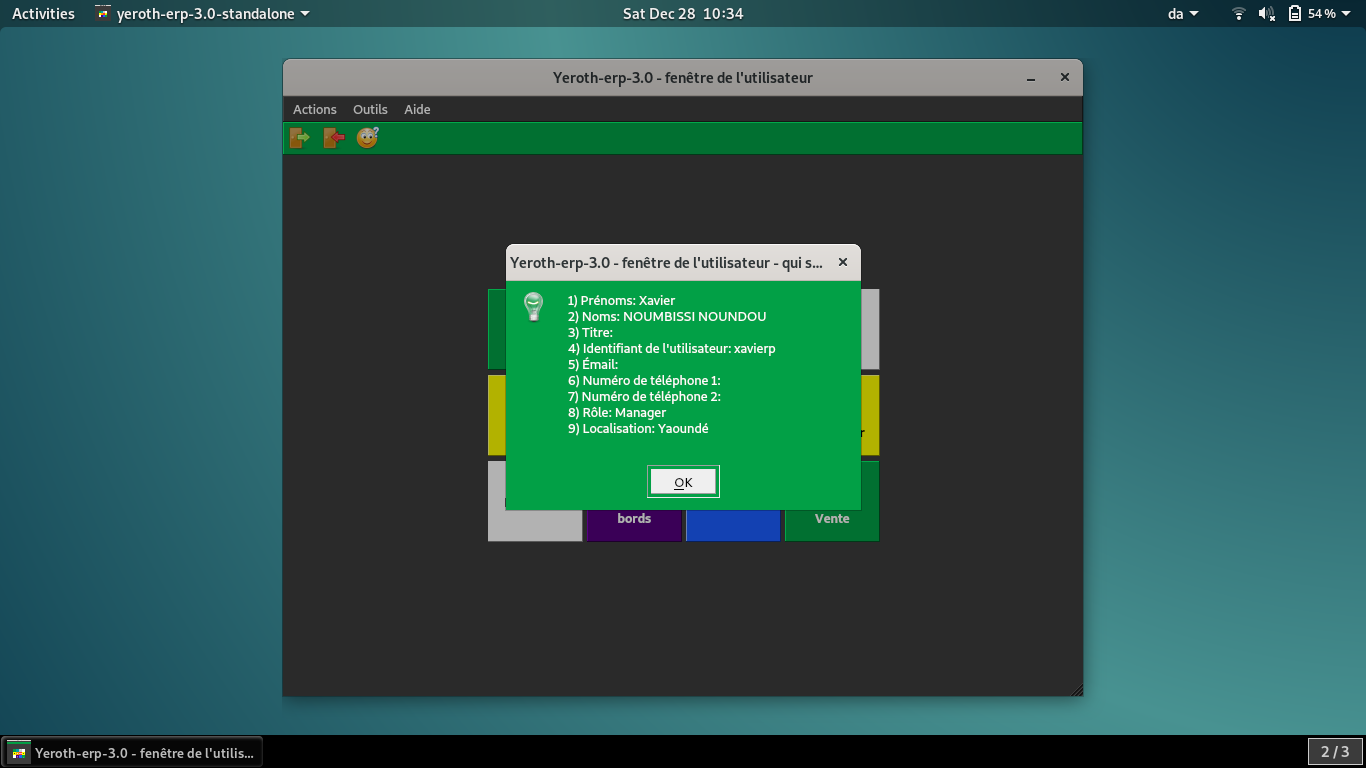
\includegraphics[scale=0.34]{images/yeren-qui-suis-je.png}
	\caption{Un example de la fonctionalit\'e 'Qui suis je ?'.}
	\label{fig:yeren-qui-suis-je}
\end{figure}

La figure~\ref{fig:yeren-qui-suis-je} illustre un example de
la fonctionalit\'e '\textbf{Qui suis je ?}'.

\`A partir de n'importe quelle fen\^etre de \yeren, cliquez
sur le lien '\textbf{Qui suis je ?}' dans le menu d\'eroulant
'\textbf{Outils}' pour obtenir les informations suivantes
de l'utilisateur avec lequel on s'est enregistr\'e:

\begin{enumerate}[1)]
	\item l'\'email
	\item l'identification de l'utilisateur	
	\item la localisation
	\item les noms	
	\item le num\'ero de t\'el\'ephone 1
	\item le num\'ero de t\'el\'ephone 2	
	\item les pr\'enoms
	\item le r\^ole	
	\item le titre.
\end{enumerate}

%---------------------------------------------------------------

\nxsection{Voir les informations g\'en\'erales de l'entreprise}
\index{voir les informations g\'en\'erales de l'entreprise}

\`A partir de n'importe quelle fen\^etre de \yeren (except\'e
les fen\^etres de l'administration), cliquez
sur le lien '\textbf{Informations sur l'entreprise}' dans
le menu d\'eroulant '\textbf{Aide}' pour obtenir les
informations suivantes de l'entreprise o\`u \yeren
est ainsi d\'eploy\'e:

\begin{enumerate}[1)]
	\item l'\'email
	\item l'adresse
	\item la bo\^ite postale
	\item la d\'enomination de l'entreprise
	\item la localisation
	\item le num\'ero de contribuable	
	\item le pays
	\item les secteurs d'activit\'es
	\item le si\`ege social
	\item le t\'el\'ephone
	\item la ville.
\end{enumerate}

La figure~\ref{fig:yeren-informations-generales-entreprise}
illustre un example de la fonctionalit\'e 
'\textbf{Informations sur l'entreprise}'.\\

\begin{figure}[!htbp]
	\centering
	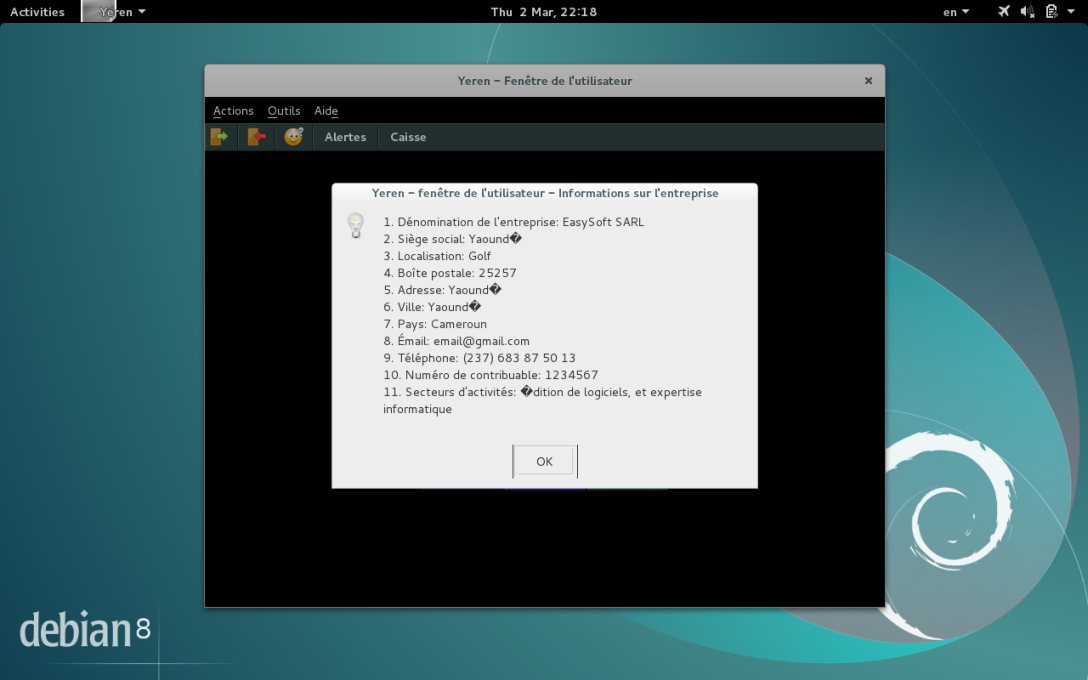
\includegraphics[scale=0.4]{images/yeren-informations-generales-entreprise.png}
	\caption{Un example de la fonctionalit\'e 'Informations sur l'entreprise'.}
	\label{fig:yeren-informations-generales-entreprise}
\end{figure}

%---------------------------------------------------------------

\newpage
\nxsection{Voir le manuel de l'utilisateur au format PDF}
\index{manuel de l'utilisateur au format PDF}

Il suffit de cliquer sur le lien '\textbf{Manuel de l'utilisateur (PDF)}'
qui se trouve dans le menu '\textbf{Aide}' de la fen\^etre
principale de chaque type d'utilisateur de \yeren:

\begin{enumerate}[1)]
	\item \admin (voir figure~\ref{fig:fenetre-principale-admin})
	\item \caissier (voir figure~\ref{fig:fenetre-principale-caissier})
	\item \magasinier (voir figure~\ref{fig:yeren-fenetre-magasinier})
	\item \manager (voir figure~\ref{fig:yeren-fenetre-patron}).		
\end{enumerate}

%---------------------------------------------------------------

\nxsection{Voir la version de \yeren que vous utilis\'e}
\index{voir la version de \yeren que vous utilis\'e}

Il suffit de cliquer sur le lien '\textbf{\`A propos}' qui
se trouve dans le menu '\textbf{Aide}' de n'importe quelle
fen\^etre de \yeren.

La figure~\ref{fig:yeren-apropos}
illustre un example de la fonctionalit\'e 
'\textbf{\`A propos}'.

\begin{figure}[!htbp]
	\centering
	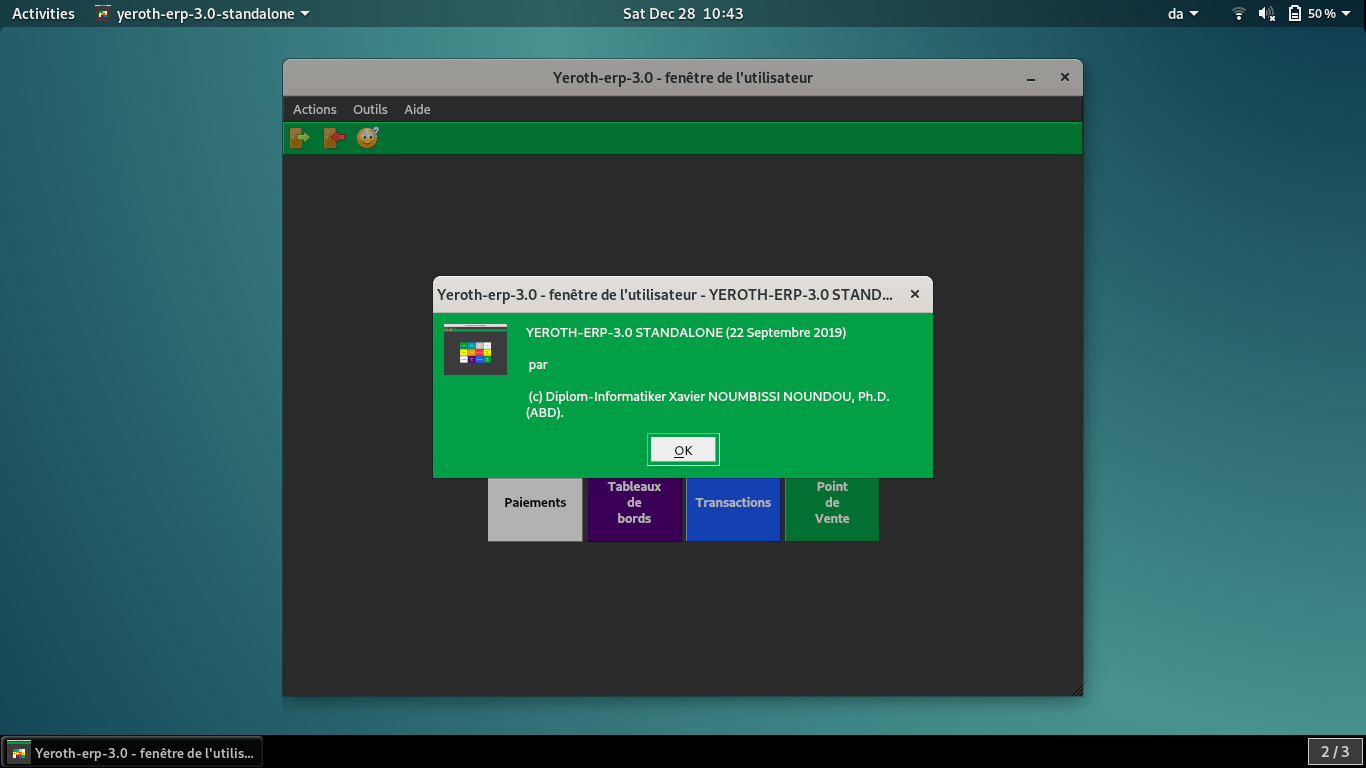
\includegraphics[scale=0.369]{images/yeren-apropos.png}
	\caption{Un example de la fonctionalit\'e '\`A propos'.}
	\label{fig:yeren-apropos}
\end{figure}


